\def\layersep{4cm}
\def\inputbegin{1}
\def\inputend{3}
\def\hiddenbegin{4}
\def\hiddenend{7}
\def\outputbegin{8}
\def\outputend{9}

\shorthandoff{<}
\shorthandoff{>}
\tikzsetnextfilename{figures/mlp/mlp}
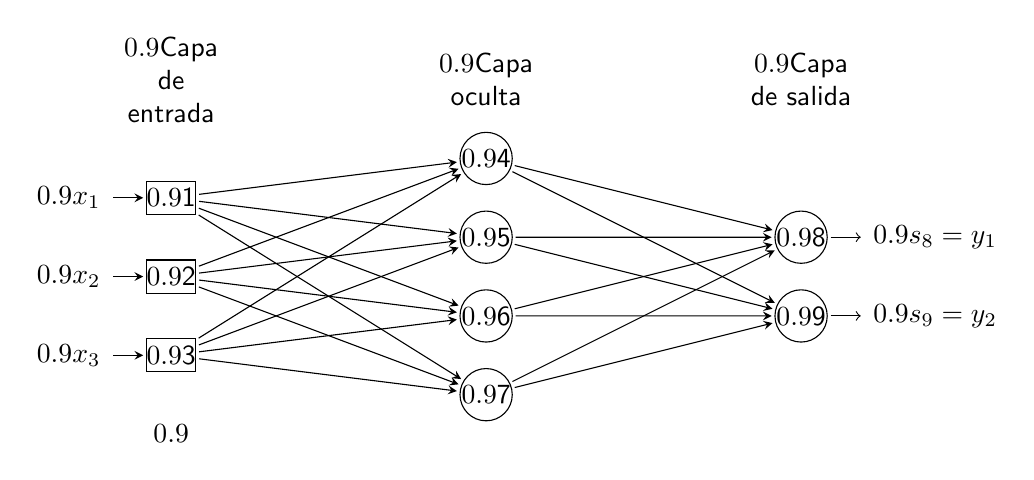
\begin{tikzpicture}[   % opciones por defecto
    shorten >=1pt,     % acortar la linea en 1pt al final
    shorten <=1pt,     % acortar la linea en 1pt al principio
    - stealth,         % estilo de flecha al final (manual pgf p~210)
    draw=black!100,    % linea negro 100%
    node distance=\layersep, % no se que hace esto
    font=\relscale{0.9}\sffamily
  ]

  \tikzstyle{every pin edge}=[stealth -,shorten <=1pt]
  \tikzstyle{neuron}=[draw, minimum size=17pt,inner sep=0pt]
  \tikzstyle{input neuron}=[neuron, minimum size=12pt];
  \tikzstyle{output neuron}=[neuron, circle];
  \tikzstyle{hidden neuron}=[neuron, circle];
  \tikzstyle{annot} = [text width=4em, text centered]

    % Draw the input layer nodes
    \foreach \name / \y in {\inputbegin,...,\inputend}
    % This is the same as writing \foreach \name / \y in {1/1,2/2,3/3,4/4}
        \node[input neuron, pin=left:{$x_\y$}] (N-\name) at (0,-\y) {\y};

    % Draw the hidden layer nodes
    \foreach \name / \y in {\hiddenbegin,...,\hiddenend}
        \path[yshift=\hiddenbegin cm - 0.5cm]
        node[hidden neuron] (N-\name)
        at (\layersep,-\y cm) {\y};

    % Draw the output layer nodes
        \foreach \name[count=\mycount from 1] / \y in {\outputbegin,...,\outputend}
        \path[yshift=\outputbegin cm - 1.5cm]        
        node[output neuron,pin={[pin edge={->}]right:{$s_\y=y_\mycount$}},%
              right of=H-3] (N-\name) at (\layersep,-\y){\y};

    % Connect every node in the input layer with every node in the
    % hidden layer.
    \foreach \source in {\inputbegin,...,\inputend}
        \foreach \dest in {\hiddenbegin,...,\hiddenend}
            \path (N-\source) edge (N-\dest);

    % Connect every node in the hidden layer with the output layer
    \foreach \source in {\hiddenbegin,...,\hiddenend}
        \foreach \dest in {\outputbegin,...,\outputend}
            \path (N-\source) edge (N-\dest);

    % Annotate the layers
    \node[annot,above of=N-\hiddenbegin, node distance=1cm] (hl) {Capa oculta};
    \node[annot,left of=hl] {Capa de entrada};
    \node[annot,right of=hl] {Capa de salida};
    \node[annot] at (0,-4) {};
\end{tikzpicture}
\shorthandon{<}
\shorthandon{>}
